\documentclass{beamer}
\usetheme{Madrid}

\usepackage{ctex}

\title{蒙特卡罗方法与哈希碰撞}
\author{祝润天}
\institute{复旦大学计算机科学技术学院}
\date{2024 年 9 月 13 日}

\begin{document}

\begin{frame}
    
    \maketitle

\end{frame}

\begin{frame}
    \frametitle{目录}

    \tableofcontents

\end{frame}

\section{蒙特卡罗方法}

\subsection{计算圆周率}

\begin{frame}
    \frametitle{计算圆周率}

    \begin{problem}
        假设有一台普通的计算机可以使用,如何计算圆周率的数值?       
    \end{problem}

    \pause

    \begin{block}{级数方法}
        $$\frac{\pi}{4} = 1 - \frac{1}{3} + \frac{1}{5} - \frac{1}{7} + \frac{1}{9} - \cdots = \sum_{k = 0}^{\infty} \frac{(-1)^k}{2k + 1}$$
        $$\pi = 4\sum_{k = 0}^{\infty} \frac{(-1)^k}{2k + 1}$$
    \end{block}

\end{frame}

\begin{frame}
    \frametitle{计算圆周率}

    \begin{problem}
        假设有一台普通的计算机可以使用,如何计算圆周率的数值?       
    \end{problem}

    \begin{block}{Chudnovsky 算法}
        $$S = \sum_{n = 0}^{\infty} (-1)^n \frac{(6n)!(k_2+nk_1)}{(n!)^3(3n)!(8k_4k_5)^n}$$
        $$\pi = \frac{k_6\sqrt{k_3}}{S}$$
        其中
        $$k_1 = 545140134, k_2 = 13591409, k_3 = 640320,$$
        $$k_4 = 100100025, k_5 = 327843840, k_6 = 53360$$
    \end{block}
    太吓人了!(也不是今天的主题)

\end{frame}

\begin{frame}
    \frametitle{投点法}

    \begin{problem}
        在边长为 $1$ 的正方形中有一内接四分之一圆。在正方形中随机取点,点在四分之一圆内的概率是多少?   
    \end{problem}

    \begin{columns}
        \column{.38\textwidth}

        $$p = \frac{S_{\text{圆}}}{S_{\text{正方形}}} = \frac{\pi}{4}$$
    
        $$\pi = 4p$$

        \column{.58\textwidth}

        \begin{figure}
            \centering
            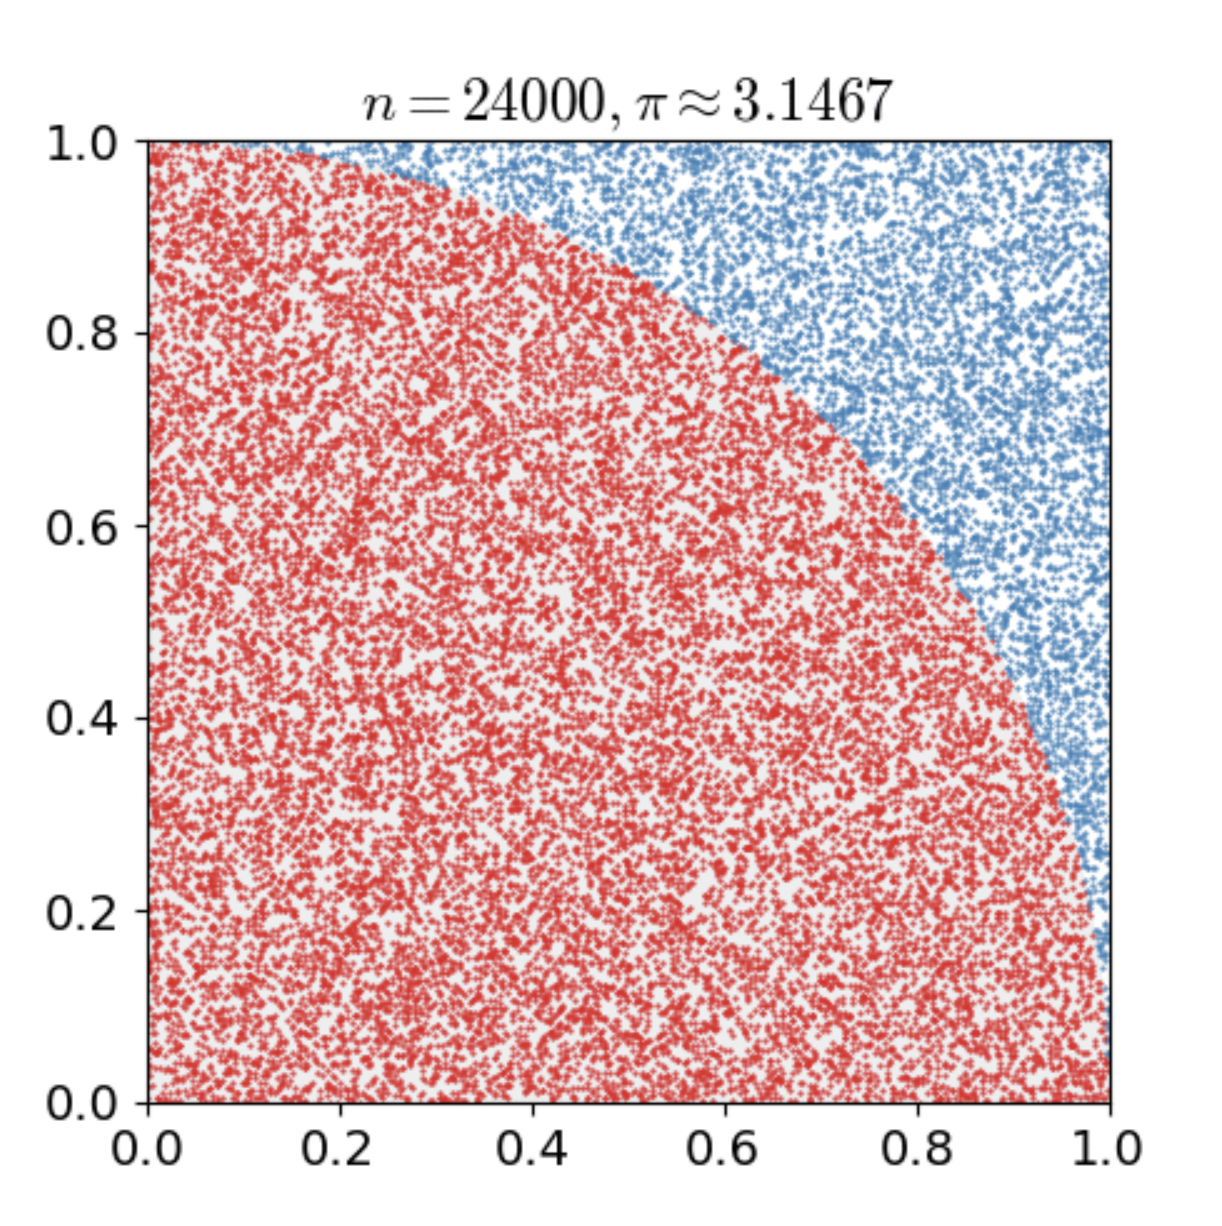
\includegraphics[scale=0.12]{res/pi_calc.png}
        \end{figure}
    \end{columns}

\end{frame}

\subsection{蒙特卡罗方法}

\subsection{计算定积分}

\subsection{光线追踪}

\section{哈希碰撞}

\subsection{生日悖论}

\subsection{哈希碰撞}

\begin{frame}
    \frametitle{<title>}

    

\end{frame}

\end{document}